\section{State of the Art}
In this section, the current IT-systems will be described and what other systems that can be used to plan what food to eat.

\section{Food Planner}
Some of the technologies that are currently being used to make a food plan could be a mobile application called Food Planner.
In this application the users can plan meals ahead of time, lookup recipes, look at what groceries that needs to be bought,
list what the user have in the fridge so the grocery list appends to the items in the fridge and more.

\begin{figure}[H]
    \centering
    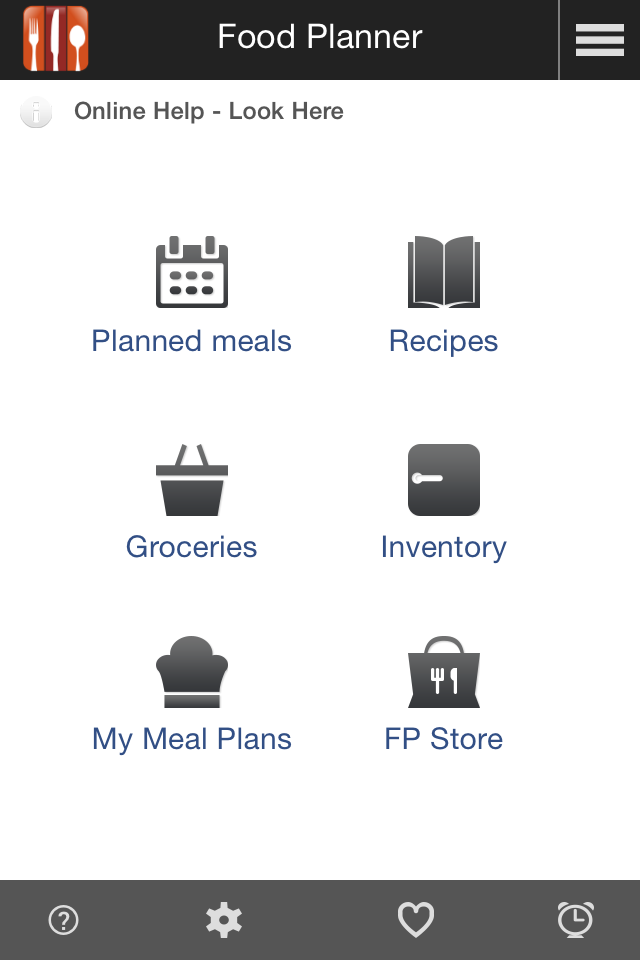
\includegraphics[width=0.5\textwidth]{Grafik/FoodPlanner/index}
    \caption{An image displaying the index of the application Food Planner}
    \label{FoodPlannerIndex}
\end{figure}

%Kan filføle flere billeder af FoodPlanner appen og uddube dem.

\section{Website}
Another alternative could be the website http://www.madplanuge.dk/madplan/lav-madplan \fxnote{Ref the website, so its not in the text?}
, where a foodplan can be planned one week ahead, but the users storage is taken into consideration.

\begin{figure}[H]
    \centering
    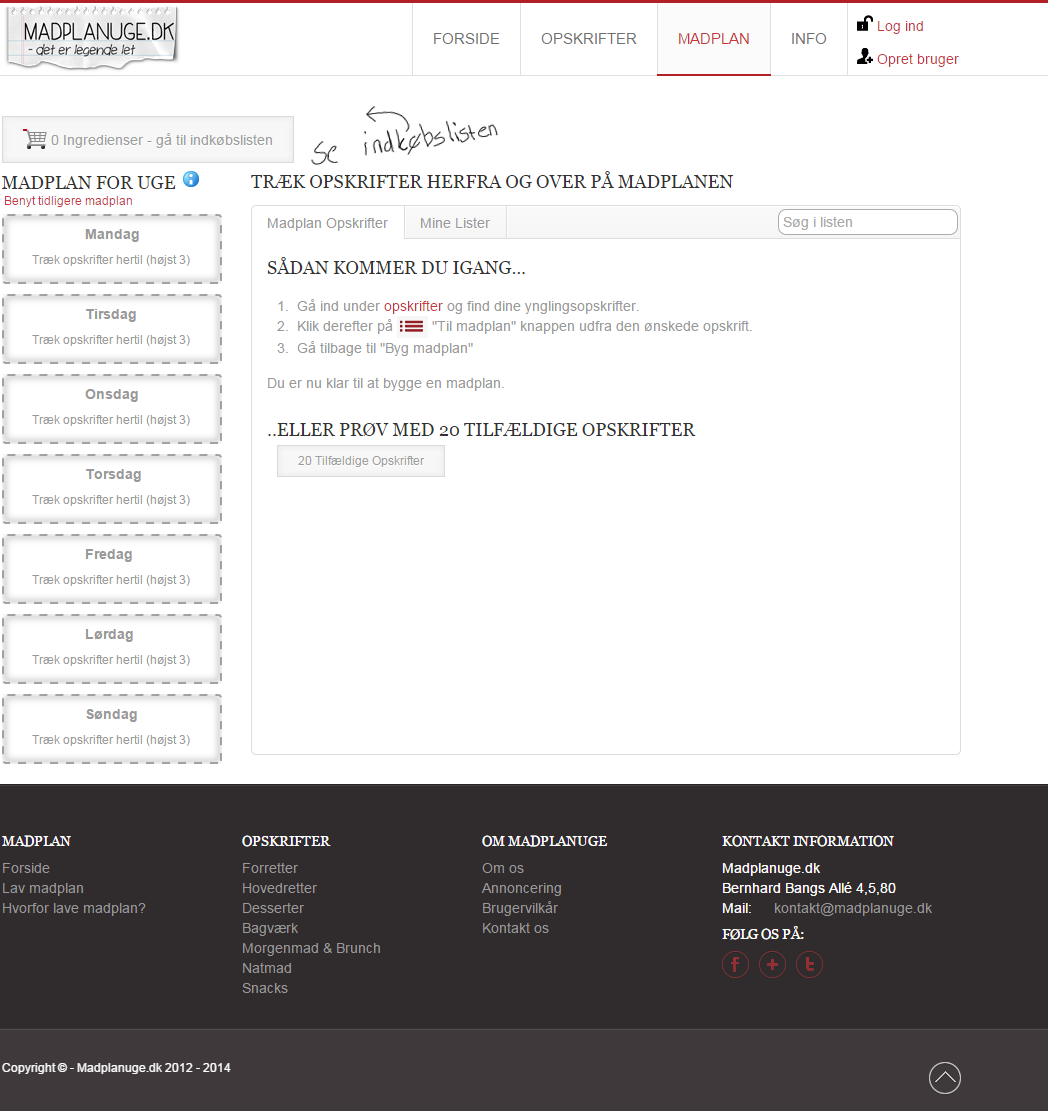
\includegraphics[width=0.5\textwidth]{Grafik/madplanuge}
    \caption{An image displaying the the website Madplan Uge}
    \label{MadPlanUge}
\end{figure}


